
\documentclass[11pt]{article}

\usepackage[margin=0.75in]{geometry}
\usepackage[english]{babel}
\usepackage{amsmath}
\usepackage[utf8x]{inputenc}
\usepackage[T1]{fontenc}
\usepackage{listings}
\usepackage[final]{pdfpages}
\usepackage{hyperref}
\usepackage{apacite}
\usepackage{soul} % Allows strikethroughs with \st
\usepackage{graphicx}
\usepackage{float}

\begin{document}
\pagenumbering{roman}
\vspace*{0.5in}

\begin{center}
\Huge{{\bf IE332 Final Project}}
\end{center}

\vspace{0.3in}

\noindent We certify that the submitted work does not violate any academic misconduct rules, and that it is solely our own work. By listing our names and student IDs we acknowledge that any misconduct will result in appropriate consequences.  Moreover, we have {\bf read and understood the assignment instructions}.

\vspace{0.2in}

\noindent {\em ``As a Boilermaker pursuing academic excellence, I pledge to be honest and true in all that I do.
Accountable together - we are Purdue.''}

\vspace{0.3in}

\begin{flushleft}
FULL name of each team member, as indicated in Blackboard:
\begin{table}[h]
\centering
\begin{tabular}{l|l|l}
Name                       & PUID       & Purdue Email Address                                    \\ \hline
Alexander (Alex) Rastovski & 0027736002 & \href{mailto:arastovs@purdue.edu}{arastovs@purdue.edu}  \\
Austin Bohlin              & 0026937790 & \href{mailto:abohlin@purdue.edu}{abohlin@purdue.edu}    \\
Blake Cobb                 & 0027886040 & \href{mailto:cobb17@purdue.edu}{cobb17@purdue.edu}      \\
Brad Johnson               & 0027867858 & \href{mailto:john1663@purdue.edu}{john1663@purdue.edu}  \\
Brandon Haberman           & 0028786526 & \href{mailto:bhaberma@purdue.edu}{bhaberma@purdue.edu}  \\
John (Jack) Penna          & 0028167175 & \href{mailto:jpenna@purdue.edu}{jpenna@purdue.edu}      \\
Jacob Moeckler             & 0028764178 & \href{mailto:jmoeckle@purdue.edu} {jmoeckle@purdue.edu}
\end{tabular}
\end{table}

\end{flushleft}

\vspace{0.2in}

\noindent Date: \today




% We created a separate file where the actual contents of Phase 1 are located.  This allows us to quickly change the input file for each phase without the worry that something has been mistakenly been edited in this file.

\renewcommand{\thepage}{}
\section*{Website}
Tested on Google Chrome and Firefox:\\

\url{https://web.ics.purdue.edu/~g1090432/}
\subsection*{Major Webpages}
\begin{itemize}
\item \textbf{Homepage} \url{https://web.ics.purdue.edu/~g1090432/}
\item \textbf{Login and register page} \url{https://web.ics.purdue.edu/~g1090432/login.php}
\item \textbf{Logout page} \url{https://web.ics.purdue.edu/~g1090432/logout.php}
\item \textbf{Space Information prior to booking} \url{https://web.ics.purdue.edu/~g1090432/www/pages/space?space=762}
\item \textbf{Booking (need to be signed in as lessee)} \url{https://web.ics.purdue.edu/~g1090432/www/pages/book.php?space=139\&startdate=2018-01-18\&enddate=2019-05-18}
\item \textbf{Lessee list of contracts (need to be signed in as lessee)} \url{https://web.ics.purdue.edu/~g1090432/www/pages/lesseeAccount}
\item \textbf{Lessee Edit Account Info (need to be signed in as lessee)} \url{https://web.ics.purdue.edu/~g1090432/www/pages/lesseeProfile}
\item \textbf{Warehouse Owner Dashboard (need to be signed in as owner)} \url{https://web.ics.purdue.edu/~g1090432/www/pages/warehouse}
\item \textbf{Warehouse Contract List (need to be signed in as owner)} \url{https://web.ics.purdue.edu/~g1090432/www/pages/contractList}
\item \textbf{Locations owned by a warehouse owner (need to be signed in as owner)} \url{https://web.ics.purdue.edu/~g1090432/www/pages/locations}
\item \textbf{@Capcity Dashboard (need to be signed in as root)} \url{https://web.ics.purdue.edu/~g1090432/www/pages/warehouse}
\item \textbf{@Capcity Contract List (need to be signed in as root)} \url{https://web.ics.purdue.edu/~g1090432/www/pages/contractList}
\item \textbf{All @Capacity Locations (need to be signed in as root)} \url{https://web.ics.purdue.edu/~g1090432/www/pages/locations}
\item \textbf{Warehouse Owner Edit Profile Page (need to be signed in as owner)} \url {https://web.ics.purdue.edu/~g1090432/www/pages/ownerProfile}
\item \textbf{Warehouse Owner Edit Warehouse (need to be signed in as root or owner)} \url{https://web.ics.purdue.edu/~g1090432/www/pages/editLocation?edit=1&warehouse=1}
\item \textbf{Warehouse Owner Edit Space (need to be signed in as root or owner)} \url{https://web.ics.purdue.edu/~g1090432/www/pages/editSpace?edit=1&space=1}
\item \textbf{Warehouse Owner Add Warehouse (need to be signed in as root or owner)} \url {https://web.ics.purdue.edu/~g1090432/www/pages/editLocation?add=1}
\item \textbf{Warehouse Owner Add Space (need to be signed in as root or owner)} \url{https://web.ics.purdue.edu/~g1090432/www/pages/editSpace?add=1&warehouse=935}
\item \textbf{Survey of Lessee (must be signed in as Owner)}\url{https://web.ics.purdue.edu/~g1090432/www/pages/Owner_Survey?contract=30}
\item \textbf{Survey of Space (must be signed in as Lessee)}\url{https://web.ics.purdue.edu/~g1090432/www/pages/Lessee_Survey_2?contract=500}
\end{itemize}

\section*{Bonus Points}
\begin{itemize}
\item Utilization of an Open Source Role Based Access Control \cite{abiusx} to separate users by roles (Root, Owner, Lessee)
\item "Sanitation" of SQL queries to prevent SQL Injections.  This has been tested with the example from lecture.  The function that sanitizes SQL injections is called "clean" and is in the file \textit{www/includes/sanitize.php} lines 1:9.  This function takes in the text needing to be sanitized and outputs the sanitized version.
\item Notifications for the Warehouse Owner for new contracts (this is a work in progress).  The notifications are on the top right of the warehouse dashboard, highlighted as red if there is a notification.
\item Utilization of Leaflet and openstreetmap.org map layer to provide the lessee with the location of the space during their search and their booking process
\item A carousel of pictures are displayed to the lessee while looking at a location to lease.  These pictures are for the entire warehouse.  To add/ remove a picture for a warehouse, this is through the Edit Warehouse page from above.
\item Utilization of javascript graphs, such as Zing 
\item Nearby results on the homepage based on browser and IP location
\item Location search is based on the Google Autocomplete Location Search API (note: Google limits the amount of queries we can send.  If the location autocomplete is not showing, this is because Google stopped our API key)
\item Passwords are md5 hashed for security in the database
\item .htaccess file preserves file organization with web pages so the root folder redirects to www/pages and .php is hidden from the url
\item contact form sends an email to our group email and the recipient email regarding the contents of the contact form
\item Presentation is made in LaTeX, the LaTeX code is included in submittal.
\item ReCaptcha is on the contact form to spam contacts cannot be created.
\item \textbf{Our group utilized GitHub and XAMPP to work on the website.  This is evidenced by the below picture displaying our finalized GitHub Repository}
\begin{figure}
\centering
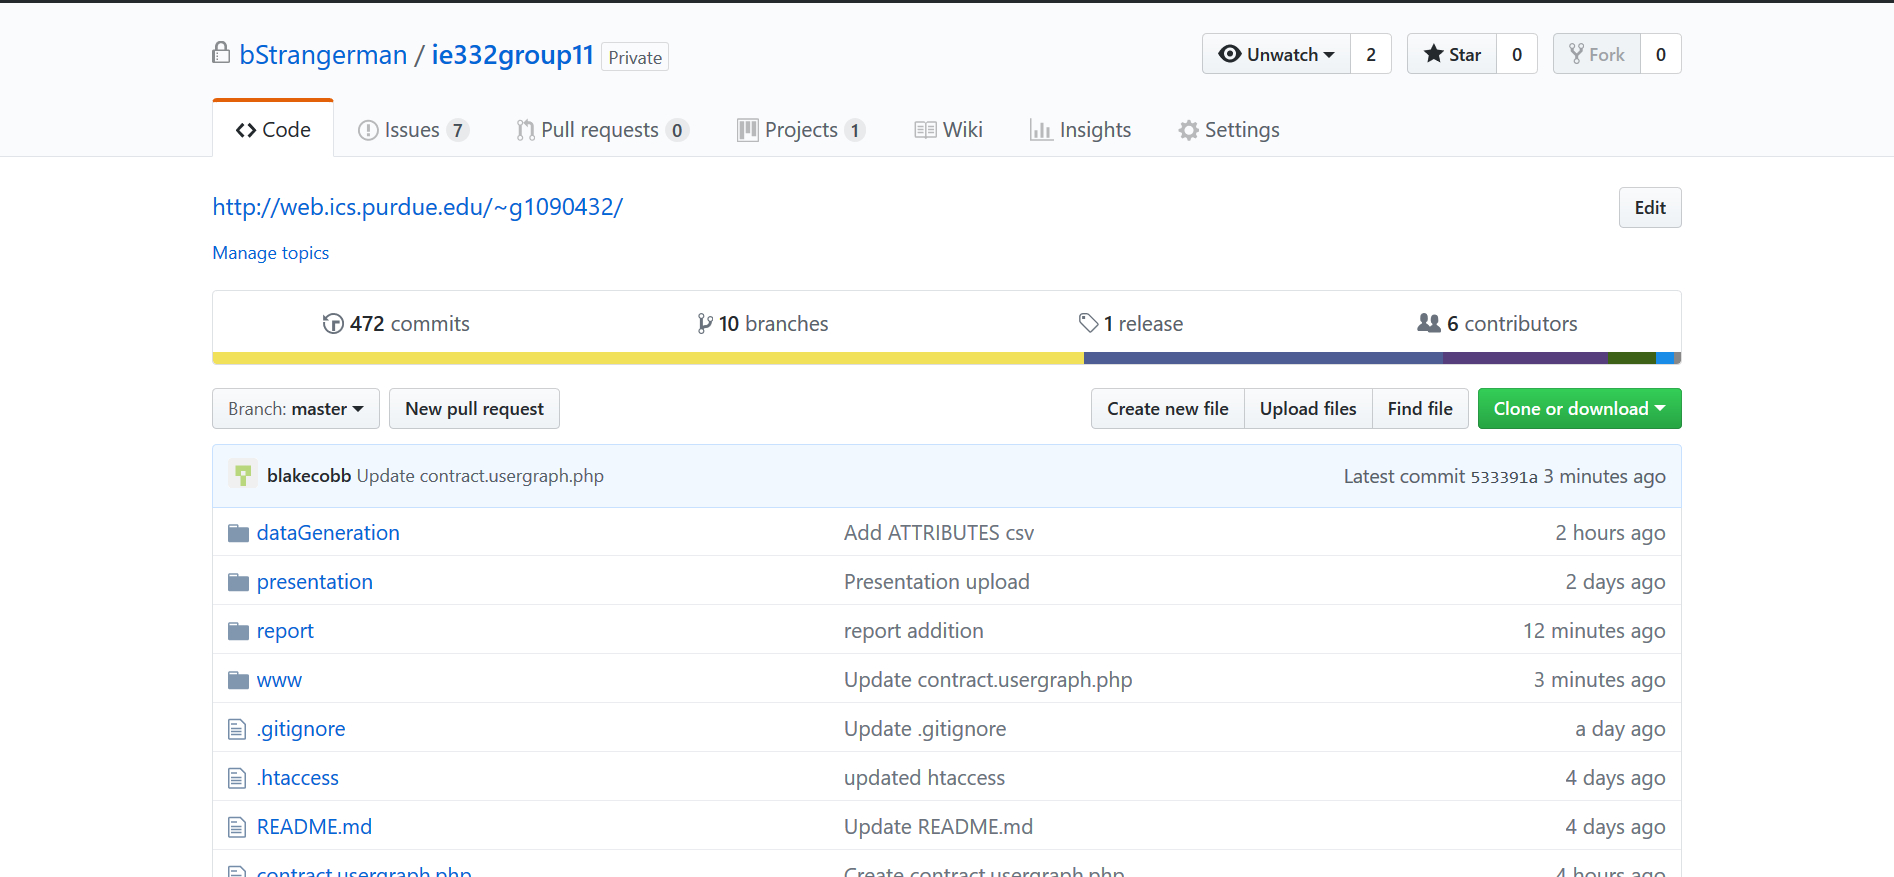
\includegraphics[width=\textwidth]{Phase_3/github}
\end{figure}
\end{itemize}

\section*{Account Information}
\begin{itemize}
\item \textbf{root} : th!sPwd!s4r00t
\item \textbf{owner} : th!sPwd!s40wner
\item \textbf{lessee} : th!sPwd!s4Le55ee
\begin{itemize}
    \item Purdue Career Account Information Username: \textbf{g1090432} / Password: \textbf{J2fujDWC}
\item Purdue SQL Account Username: \textbf{g1090432} / Password: \textbf{@Capacity332}
\begin{itemize}
\item When modifying the SQL Account information, modify 
\begin{itemize}
\item www/includes/db.php
\item www/includes/PhpRbac/database/database.config

\end{itemize}

\end{itemize}
\end{itemize}
\end{itemize}

\newpage
\tableofcontents
\newpage
\pagenumbering{arabic}

\section{Overview}
One of the largest issues in the warehouse space industry is the lack of relationships between owners and future lessees that results in underused warehouses. The team memebers of @Capcity came together to form a secure solution to this hindering underuse problem for both of these parties involved by giving the lessees the flexibility to find their ideal warehouse, and better utilizing the space of warehouse owners. The core of the @Capcity Solution lies in the website's strategic search executed by the lessees to find the ideal warehouse in the ideal location. The search uses different warehouse spaces specifications and utilization features of the warehouse spaces to provide a strategic list of warehouses yielding an optimal solution for both warehouse owners and future lessees. The @Capacity team is an intriguing company to invest in due to the low risk start up costs, and self-sustaining business model. 

\section{Introduction}
A growing trend across multiple industries is the peer-to-peer sharing of resources in exchange for monetary compensation. The idea that our company, @Capacity, seeks to handle is applying this concept to the problem of underutilized warehouses. Not only are unused warehouses a waste of space, but they could easily be used by a potential lessee if the knowledge of the warehouse's existence and specifications were easily accessible. There are two main stakeholders pertaining to this issue: warehouse owners and potential lessees. Warehouse owners, of course, have the problem of having many of their warehouses go underutilized. In addition, it is difficult for owners to manage and maintain multiple warehouses, and it is hard to find one-to-one relationships with lessees with whom they could continuously partner with. On the lessee side, it is difficult to find storage space for unique requirements, and it is a tedious process to sort through information on multiple warehouses to find one with the desired specifications. Therefore, the goal is to provide warehouse owners and potential lessees a platform to efficiently search for and form 1:1 relationships that minimizes underutilized space and maximize customer satisfaction. The solution is @Capacity, a peer-to-peer warehouses sharing company that allows customers to find warehouses and lessees via the @Capacity website.

\vspace{80px}
\begin{figure}[H]
\centering

\includegraphics[width=.65\textwidth]{Phase_3/Capacity_Logo_Trans.png}
%\caption{@Capacity}
\label{fig:@Capacity}
\end{figure}

\pagebreak
\section{@Capacity Solutions}
\subsection{Flexibility and Freedom}
One of the most prominent aspects of the Voice of the Customer that led the project team to start this company was the tedious and constricting process future lessees go through in finding a warehouse. When a future lessee needs a space for storage, the first instinct is to search the web, which leads to many irrelevant results. In the Figure~\ref{fig:screenshot} below there is a screenshot of what a typical internet search would show a lessee in need of a warehouse with bay doors in Missoula, Montana. The most popular item listed in the website search is an irrelevant source that is not to going to be helpful to the lessee. 

\begin{figure}[H]
\centering
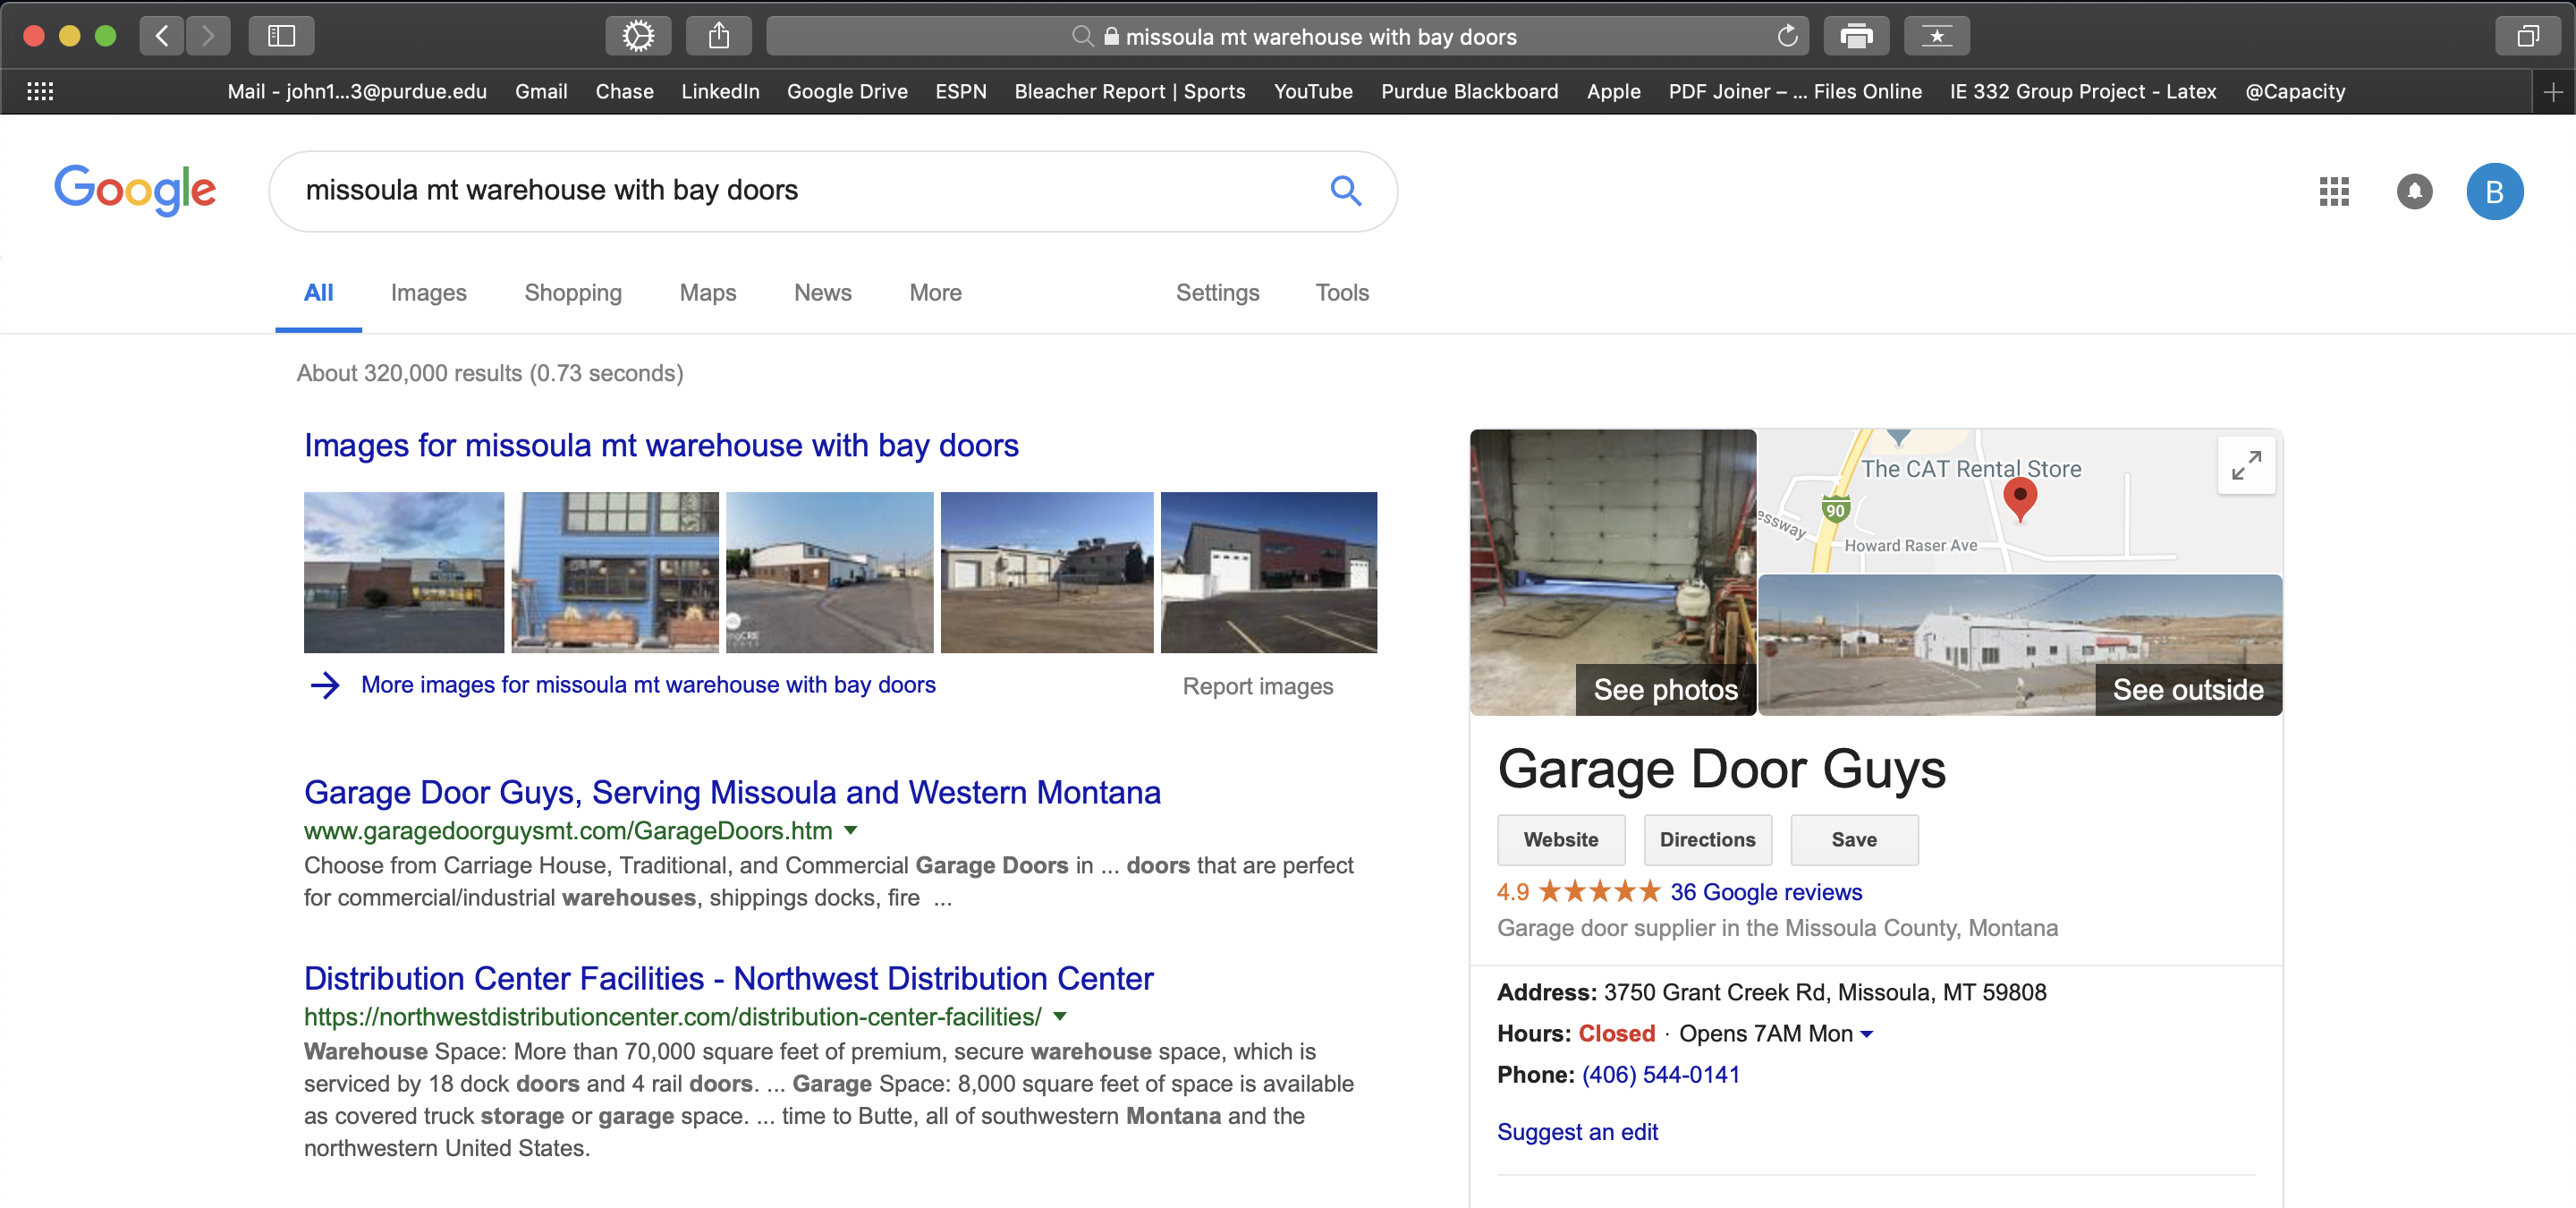
\includegraphics[width=.75\textwidth]{Phase_3/screenshot.png}
\caption{Google search results for a desired warehouse}
\label{fig:screenshot}
\end{figure}

Figure~\ref{fig:loading} shows what a quick search on the @Capacity would give a lessee. This solution provides these future lessees the flexibility to tell us what they want to store, where they want to store, and when they want to store it.  

\begin{figure}[tbh]
\centering
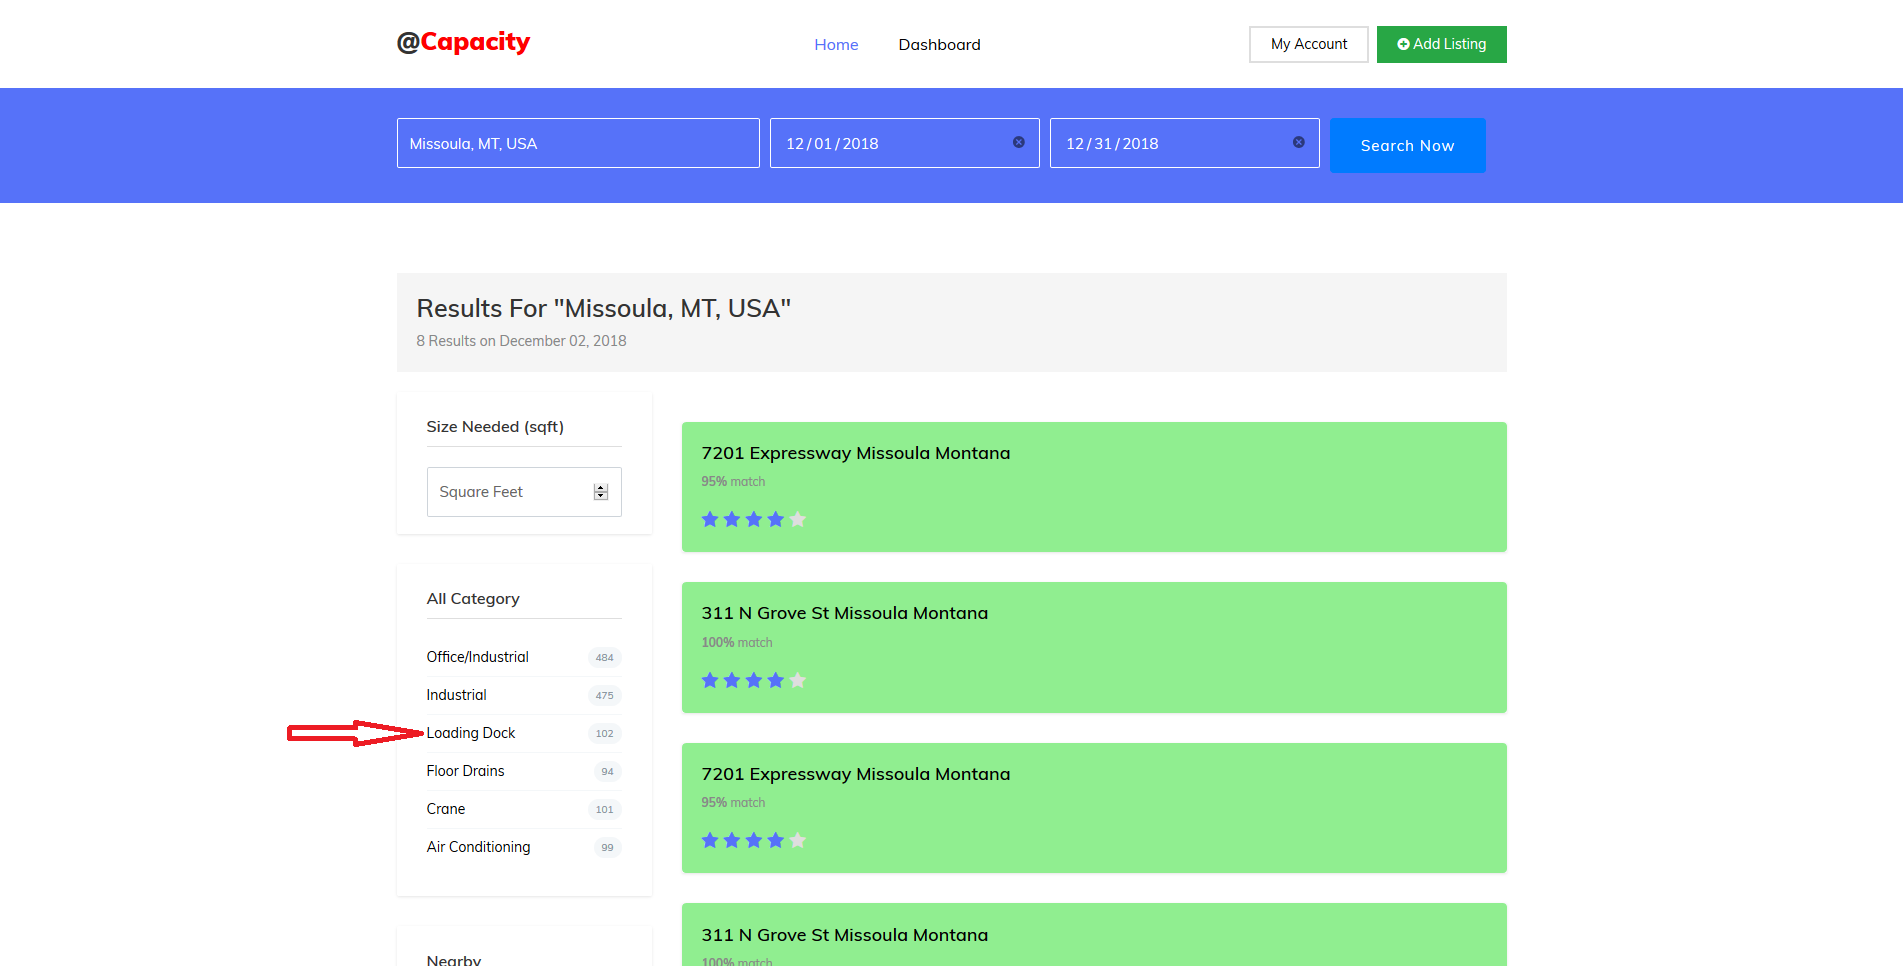
\includegraphics[width=.75\textwidth]{Phase_3/loading}
\caption{Search results from @Capacity website with the same search input as Figure 1}
\label{fig:loading}
\end{figure} 

Overall the website delivers a concise, organized list of warehouses fitting the lessee's criteria. @Capacity also provides flexibility to owners as well. Owners are given the power to control which lessees sign contracts to lease out their space. Whenever a lessee submits a contract proposal for a warehouse space the warehouse owner is given the power to accept, or decline any proposal.

  
\subsection{Quality Control}
@Capacity values giving both owners and lessees the power and ability to rate their experience in every contract they are in. Similar to the reason why consumers check the internet for reviews before they eat at a restraunt, @Capacity wants to give both owners and lessees the radical transparency in their decision making. Whenever a contract ends, both the owner and the lessee have the power to rate the overall experience both parties had in the form of a survey. The owners can rate their experience with the lessees through a singular 1-5 rating, as well as a short written survey. The lessee's survey is a bit more layered, with several more questions. The survey taken by the lessee allows them to give a 1-5 rating to five different categories in addition to a written survey. The lessee is given a little more freedom in this aspect since their experience in the transaction extends beyond the communication with their partner into the actual stay in the warehouse, as opposed to the owner's limited exposure to the rental instance. Ratings for each space and for each lessee are compiled into an overal five star rating which then can be viewed by other users. This rating system allows all users of @Capacity to have full confidence in engaging in future contracts.
\subsection{Intuitive and Informative Interface}
A solution is not worth making if it is a hassle to use. This is why one of the largest focuses with @Capcity's solution is to create a product that is as straightforward and intuitive as possible. Some of these features include:
\begin{itemize}
\item Easy registration process for owners and lessees
\item Simple-to-use dashboard to manage one's analytics
\item Thousands of warehouses available with an easy search feature for customized locations and amenities
\item @Capacity's wide range of capabilities include the ability for warehouse owners to lease spaces owned by other warehouse owners.  Through this option, users do not need to create new accounts to lease spaces.  This solution is unique to @Capacity because solutions, such as Loopnet.com, require users to have only one role.
\end{itemize}

\section{Website Features}
\subsection{Matching}
The @Capacity solution is centered around the dynamic matching system. This solution works by strategically intertwining main aspects of the warehouse spaces and aligning the ideal spaces with the warehouse needs. The four main components of the warehouse spaces include: utilization, building specifications (distance, size, price, amenities), and scheduling to match exactly what the lessee needs. 

\subsubsection{Utilization}
@Capacity's unique matching system aligns with the mission of @Capacity, to minimize underutilized warehouse space. In essence, the goal is to ensure that all owners that are leasing out their space on @Capacity's website have as close to an equal chance of being seen in the website's search function as possible. In Figure~\ref{fig:utilization2} below you will see a screen shot of a search being done in West Lafayette, IN. The two green boxes that appear in the search both fully satisfy the needs of the lessee. The reason the top search has a higher match percent is because it is less utilized then the warehouse below it, with the the hope that ultimately this space will receive the same traction as the search below it. 
\begin{figure}[tbh]
\centering
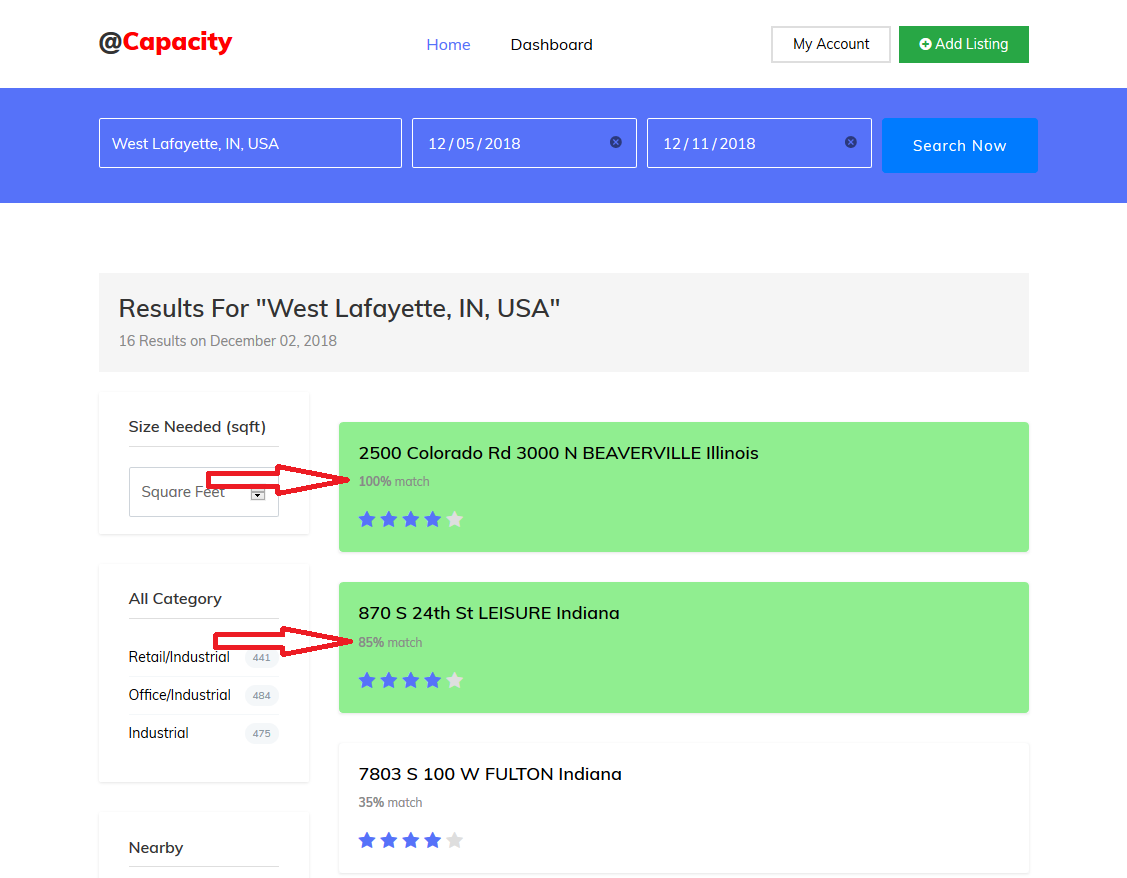
\includegraphics[width=.75\textwidth]{Phase_3/utilization}
\caption{Search results highlighting the priority given to the equally relevant less utilized warehouse}
\label{fig:utilization2}
\end{figure}


\subsubsection{Building Specifications}
\paragraph{Distance}
@Capacity's solution to matching lessees to warehouses begins with the location.  Through a search capable of probing the entire United States, the lessee is presented with a list of solutions in or near the location they searched.  Represented in Figure~\ref{fig:distance}, a search for the city, West Lafayette, provides the lessee with search results near West Lafayette, including results in Indiana and Illinois. Other indicators such as a zip code may be used to narrow down search area as well. When all parameters are inputted, the warehouse results listed will all have a percentage score communicating roughly how well this property adheres to the set of requirements

\paragraph{Size}
The minimization of underutilized space is a fundamental backbone of @Capacity and the matching to align lessee's with spaces.  The desired size of the warehouse space is a vital to the customer needs as they are aware of the total area they will need to safely store their items. @Capacity's design gives the user the option to enter their minimum size they need for the warehouse. Through @Capacity's search functionalities, results that meet and exceed a lessee's required size are given a lower matching score than a space that perfectly aligns with the required size.  For example, if a lessee requires a space of 1000 sq.ft, a result of 1500 sq.ft will have a higher match score than the result of 5000 sq.ft.  This promotes an optimization of warehouse space through minimizing unused warehouse space leased by the lessee.

\paragraph{Price}
@Capacity devised a scheme where the lessee is able to input the maximum price they are willing to spend on their space for the entirety of their rented time. In order to fully satisfy the customer, the top warehouse results will be ones either at or below their set maximum price. In the possibility there are no warehouses available below the lessee's desired price, the results will display warehouses as close to the maximum cost chosen by the user. The price is not a necessary requirement for the lessee to enter when searching for a warehouse which provides results weighted towards their other needs, regardless of the cost set by the owner. 

\paragraph{Amenities}
There are a number of different factors that differentiate warehouses across the country. @Capacity gives the lessee the ultimate freedom to search for ideal warehouses that fit their needs. Having the correct amenities can make an experience. An accessible drop down list allows users to select what amenities they would like. The page will then update with available warehouses that match as close as possible to the amenities wanted. 


\subsubsection{Scheduling}
Finding the perfect warehouse is only part of the matching process. Whan a lessee is looking for a space the time this space is available is an essential component in the decision process. On the @Capacity website the lessee is prompted to enter the dates they are looking for before they are shown any spaces. The reason the search occurs this way is the @Capacity team finds it inefficient and tedious for a lessee to have to sort though any spaces that do not have the time requirements needed. In the matching solution, the desired contract time span is paired with the preferred amenities and location of the lessees choice to create an optimal and easy to read list of warehouses that should fit the lessees needs.  


\begin{figure}[H]
\centering
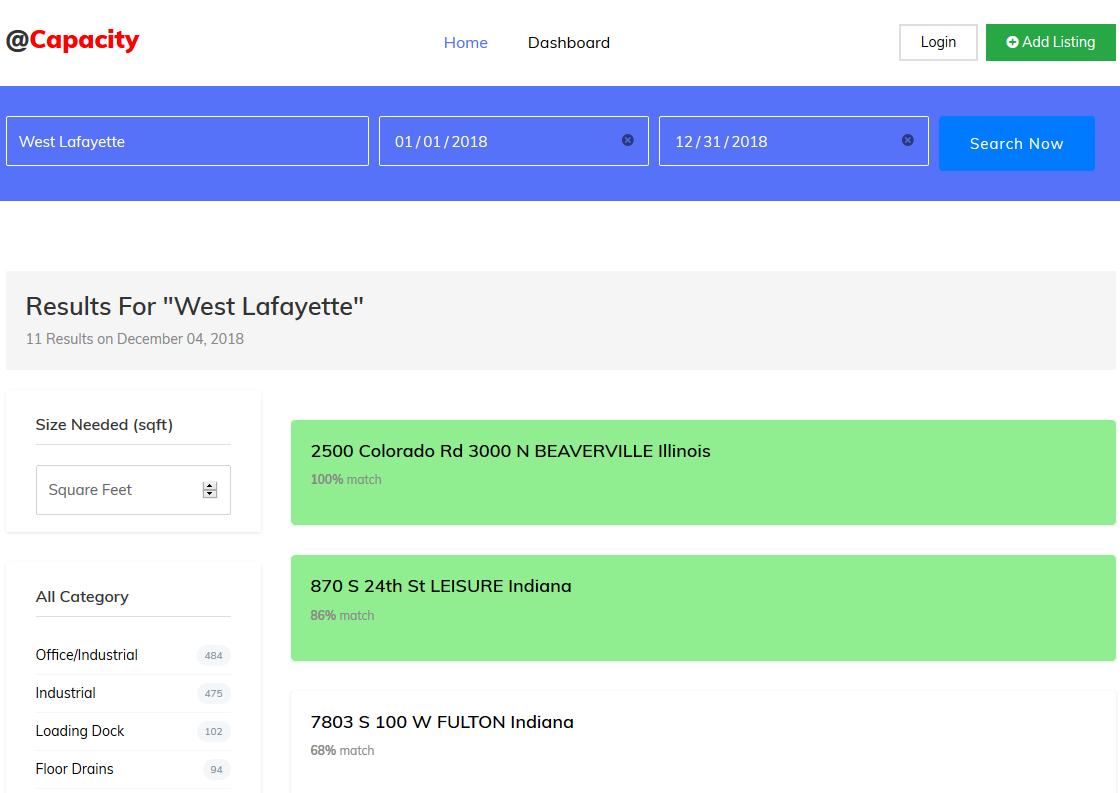
\includegraphics[width=.75\textwidth]{Phase_3/distance}
\caption{Results of the distance based search for West Lafayette}
\label{fig:distance}
\end{figure}

\subsection{Analytics}
Several key dynamic data points are established as indicators of growth and stability. As seen below in Figure~\ref{fig:ownergraph} @Capacity allows the owner of a warehouse to track revenue over time and indicate trends in market demand or development for discrete areas. @Capacity also gives owners the tools to manage properties as a part of a larger portfolio, comparing warehouses as percentages of total investment with the company. Profit derived from the 5 \% commission is updated live based on national rental activity.
\begin{figure}[H]
\centering
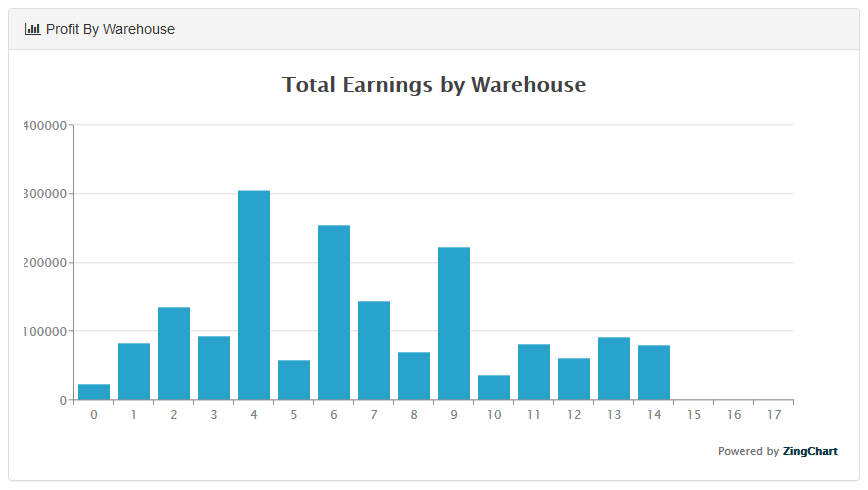
\includegraphics[width=1\textwidth]{Phase_3/earninggraph}
\caption{Snapshot in Owner's dashboard displaying total earnings for each warehouse}
\label{fig:ownergraph}
\end{figure}

\subsection{Rewards and Incentives}
As a company in touch with its users, it is in the best interest of all parties involved to reward exceptional use of the provided services. Benchmarks are established at earnings milestones influenced by occupation rates in the surrounding area. Reaching these marks allows the warehouse owner the opportunity to potentially renegotiate fee percentages for future contracts. Encouraging optimal use of warehouse services brings power users and new owners alike a new type of drive and relationship with their listing company, increasing customer retention. 



\begin{figure}[H]
\centering
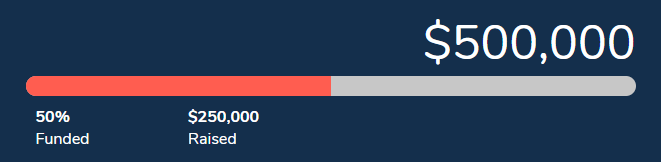
\includegraphics[width=.75\textwidth]{Phase_3/thermometer}
\caption{Reward and Incentive based Thermometer located in Owner's Dashboard}
\label{fig:thermometer}
\end{figure}

\subsection{Security}
Warehouse owners and lessees having trust in @Capacity and the solution the team provides is a pivotal point of emphasis for the company. The trust in the @Capacity team is earned in a cybersecurity manner, and through fair and proper utilization of warehouse spaces. In regards to cybersecurity, there is the proper security put in place in the forms of a payment portal, password encryption and an unauthorized access feature to ensure all users private information is kept private. The team is also intentional in using matching functionalities to optimize underutilized warehouse space providing fair representation in all warehouse space searches. 

\paragraph{Payment Portal}
@Capacity does not have, store, or need customer credit card numbers or banking details.  @Capacity completes all payment transactions through PayPal, ensuring a secure passage of payment between @Capacity and its shareholders. Paypal is an established and trusted payment platform, offering familiarity and ease of use to customers and streamlining the rental process. 

\paragraph{Passwords}
@Capacity does not know user passwords.  Through password encryption, users will have the peace of mind that their account information is safe and secure with @Capacity.  @Capacity is currently working to develop a password recovery feature and a two-step verification system to promote user satisfaction and to reduce malicious login attempts.

\paragraph{Unauthorized Access}
@Capacity commits to preventing and protecting against unauthorized access and malicious attacks against @Capacity's web service.  Through Role-Based Access-Control, @Capacity controls the pages that users can and cannot access \cite{abiusx}.  Therefore, lessees will not be able to modify warehouse information or access @Capacity's internal company dashboard.  Moreover, malicious attacks through forms and URLs exposing sensitive user information, or deleting user and company information have been throttled to strive for excellence in online security and user satisfaction.

\section{Financial Impact}
@Capacity is an intriguing company for investment due to it being centered around a low risk startup that relies on a dynamic business model. The @Capacity solution features a fully functional website, low startup cost, a self-sustaining business model, and a business structure designed for a relatively quick return on investment. The established database structure is focused on scalability and efficiency, keeping company assets directed towards revenue margins. 

\subsection{Low Startup Cost}
The leading sales pitch @Capacity has as a company is that they have a very low startup cost, which means there is a very low risk for investors. The way the team has worked towards making this happened is by completely developing the front end and the back end of the website. Therefore, the website is fully operating and the @Capacity solution is fully functional, simply waiting on it's official launch to begin to service warehouse owners and lessees.
\subsection{Self-Sustainment}
The @Capacity business model centers around the concept of being self sustaining. The thought being that the @Capacity solution has the power to handle all the searches, relationship matching, and contracts needed in the solution. Therefore very little upkeep is needed from the @Capacity team once warehouse owners and lessees join the site. 
\subsection{Business Structure}
Once the solution is fully up and running, the return in investment will begin relatively quickly. With every contract that is signed, @Capacity receives 5\% commission on each of the contracts. The most important aspect to the business, however, revolves around the ability to keep customers coming back. One of the methods @Capacity uses is making the owners feel like a valued part of the business. This is done by adding features such as a rewards program that gives the owners an incentive to continually sign contracts. The rewards program sets an annual goal for the owner to reach. If met, the owner is elgible for a reward. This annual goal tracker pairs with other dynamic features that are in the owner's dashboard to create a powerful user experience. Another feature included is tools for owners to track their profits and their space utilization. Due to the conveince and usefulnees of the dashboard, owners will develop a certain level of dependence on the @Capacity solution. In making customers dependent on the solutions environment, the @Capacity team can establish itself as a vital part of the warehouse industry and each warehouse owner's business. 

\section{Final Remarks}
@Capacity prides itself on delivering the best solution to its customers and facilities. Many features are available to both the owners and lessees that separate the company from competitors. With a secure, efficient and user-friendly website, it has never been easier to match an owner with a lessee. @Capacity has a self-sustaining business structure with a low risk startup that catches investors' eyes. Next time you need someone to lease your warehouse, make sure you work with this team, and @Capacity will keep your warehouse at capacity. 


% \appendix

\section{Database Design}

\begin{figure}[tbh]
\centering
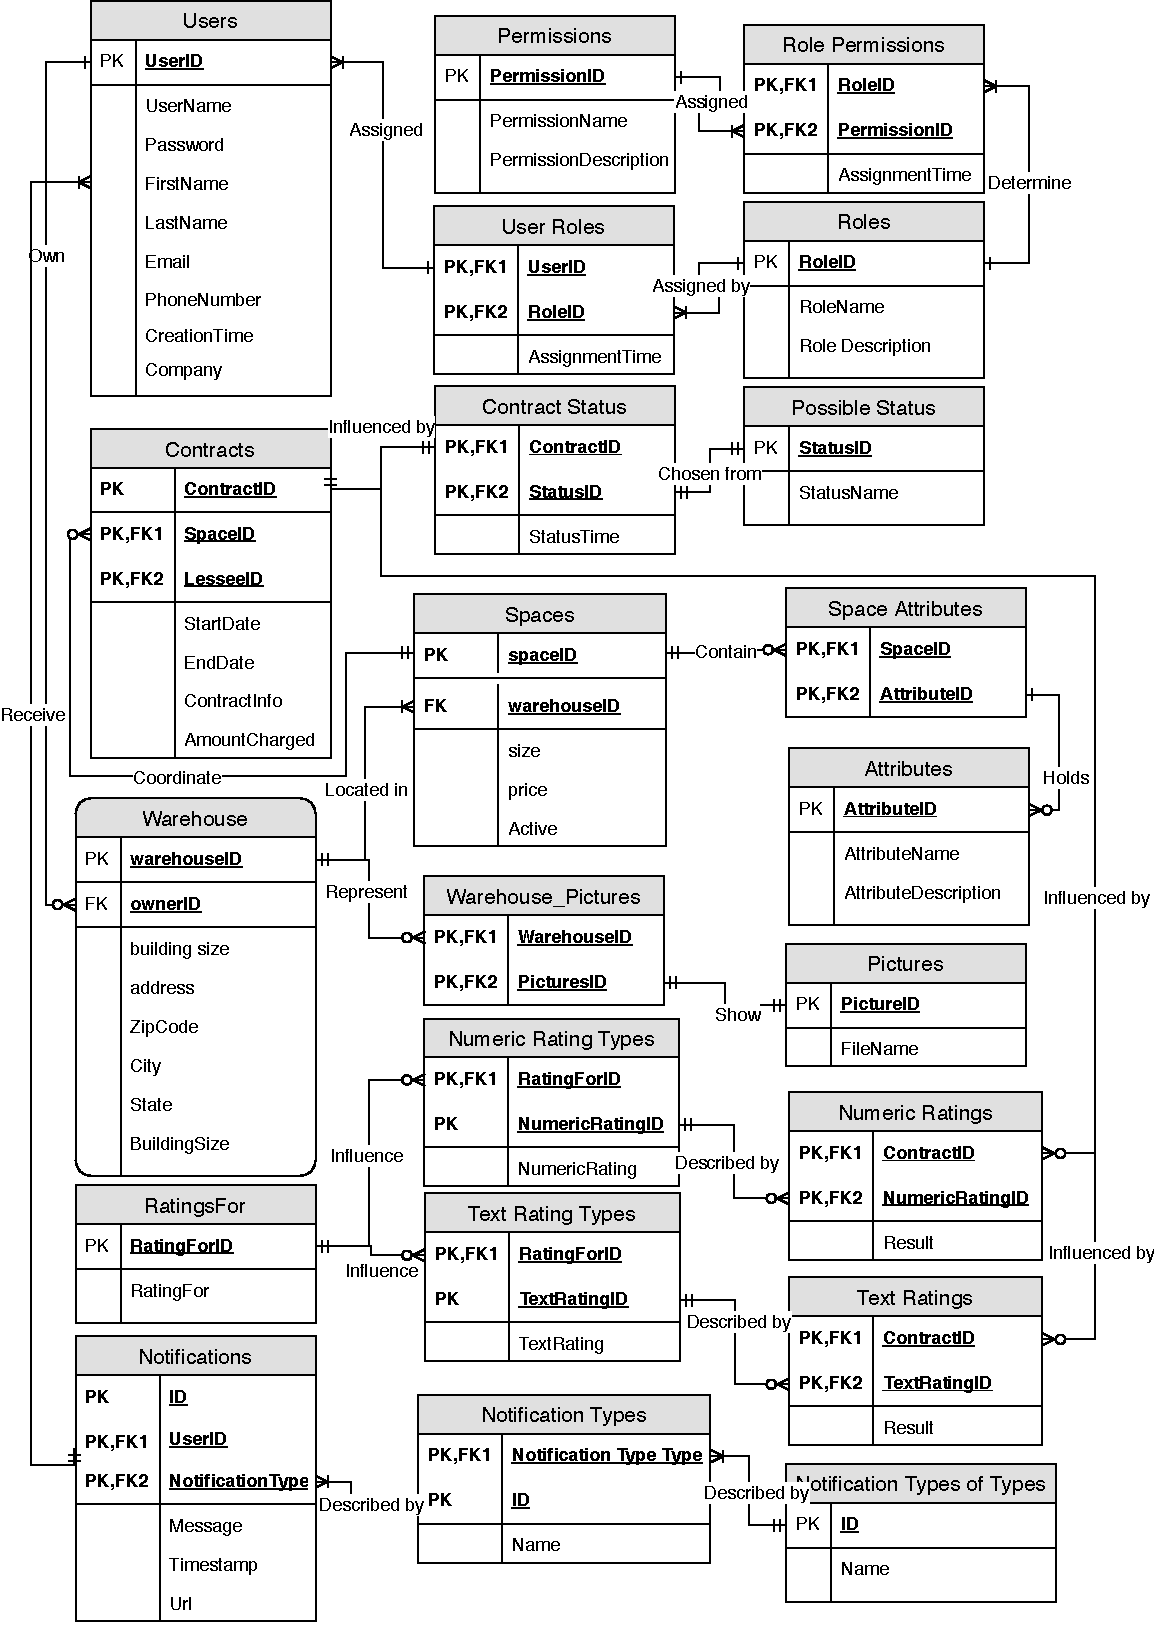
\includegraphics[page=1,width=.85\textwidth,height = .7\textheight]{Phase_3/ER_Diagram.pdf} 
\caption{Entity-Relationship Diagram}
\end{figure}

\pagebreak
\section{Ranking Algorithm}

\subsection{Utilization}
The ranking algorithm's dependency on utilization considers all the previous and future contracts for a designated space.  Utilization is divided into two parts, future utilization and past utilization.  The utilization equation is displayed in Equation~\ref{fig:utilization}.  This equation take the proportion between the time until or since the contract over the length of the contract.  This strategy promotes spaces that have not had a contract in a long time, and spaces that have shorter contracts.  Therefore the algorithim distributes contracts to a greater portion of the @Capacity community because this algorithm will distribute a higher score to less used space spaces.


\begin{figure}[h]
\[\text{Utilization} = \frac{\text{Time Until or Since the Contract}}{\text{Contract Length}}\]
\caption{Utilization for Contracts}
\label{fig:utilization}
\end{figure}


\subsection{Score}

The total score used by the ranking algorithm is a composite of 4 scores: distance, price, utilization and size.  Each one of these scores has an associated scale factor that can be changed based on the importance of each factor.  By default all the scores are scaled the same.  The total score is a simple weighted addition of each of the 3 factors as described below.



\subsubsection{Distance}

The distance score is calculated on line 287-297 in the "www/includes/rankingFunctions.php" file.  Distance\textunderscore away is a measure of how far away a given warehouse is from the clients given location.  Max\textunderscore distance\textunderscore wanted is maximum distance away a client wants their potential warehouse.  The equation below gives a linearly decreasing score to each warehouses based on its distance from the client defined location.  

\begin{figure}[h]
\[\mathrm{distance\_ score\ }=\mathrm{\ scale\ }\ast\ \left(1\ -\ \frac{(\mathrm{distance\_ away})}{(\mathrm{max\_ distance\_ wanted})}\right)\]
\caption{Distance ranking score}
\label{fig:dist}
\end{figure}

\subsubsection{Price}

The price score is calculated on line 322-326 in the "www/includes/rankingFunctions.php" file.  Space\textunderscore price is the cost of a given space.  Min\textunderscore price is the price of the cheapest space that fits the client's needs.  Max\textunderscore price is the price of the most expensive space that fits the client's needs.  The equation below gives the most expensive warehouse a score of 0, the least expensive a score of 1, and every warehouse in between a linear score between 0 and 1.

\begin{figure}[h]
\[\mathrm{price\_ score}\ =\mathrm{\ scale\ }\ast\left(1\ -\ \frac{\left(\mathrm{space\_ price\ }-\mathrm{\ min\_ price}\right)}{\left(\mathrm{max\_ price}\ -\ \mathrm{min\_ price}\right)}\right)\]
\caption{Price ranking score}
\label{fig:price}
\end{figure}

\subsubsection{Size}
The size score is calculated on line 299-320 in the "www/includes/rankingFunctions.php" file. Space\textunderscore score is the score given for each space in a warehouse. Max\textunderscore size represents the max size that each individual space has available for rent. Space\textunderscore size is user inputted value for their desired space size. This equation gives a linearly decreasing score to each warehouses based on its difference from the lessee defined size.  

\begin{figure}[h]

\[\mathrm{size\_ score}\ =\text{scale} * (1-\frac{\text{SpaceSize} - \text{SizeWanted}}{\text{MaxSpaceSize}})\]
\caption{Size ranking score}
\label{fig:size}
\end{figure}
\newpage
\section{Synthetic Data Generation}

\textbf{Contracts Pseudocode}
\\The code pertaining to the following pseudocode can be found on lines 302-362 on the file FINAL DATA GENERATION.R within the dataGeneration folder
\begin{enumerate}
\item Designate how many contracts are to be generated.
\item Generate a random number between 1 and 1400 (1400 being the number of spaces) to assign a space ID to each contract that is to be generated. 
\item Generate a random number between 350 and 1000 (this range being the range of lessee user IDs) to assign a lessee ID to each contract that is to be generated. The reason the random number is generated between 350 and 1000 is because 400-1000 are lessee user IDs, 1-350 are owner IDs, and 350-400 is a mixture of lessee and owner IDs.
\item Sort all space IDs in increasing order.
\item For each contract, if the current space ID is equal to the previous space ID, set the contract's start date equal to a random date that is greater than or equal to the previous contract's end date.
\item If the current space ID is different than the previous space ID, set the current contract's start date to a random date.
\item Set the end date for each contract to a date greater than the start date by a random number of days ranging from two weeks to two years.
\item Calculate the amount charge: for each contract, multiply the space's price/square foot/month by the length of the contract in months, the space's size, and the service fee.
\item Generate the contract information for each contract by pulling one string of random storage information from a list of storage items.
\item Compile the space ID, lessee ID, start date, end date, amount charged, and contract information into a data frame.
\item Write the contract data to a CSV file
\end{enumerate}
An important aspect to synthesizing random data that is also realistic is creating realistic contracts, as contracts are the entity that tie the space and lessee together. A realistic contract is a contract that is assigned to a particular space and lessee, does not overlap with another contract in the same space, lasts for a reasonable time, has a price calculated based on size and time, and contains information on what is being store. For this data, each contract is assigned to a space and lessee randomly using a simple "sample" function over the range of possible values for each attribute. The price is calculated using the space price and space size calculated during the space data generation. In this case, it was important to ensure that the price and size that were being used in each contract's price calculation corresponded to the space that the contract was being assigned to.\\
\\Another extremely important issue in creating realistic contracts was the scheduling aspect. As previously stated, realistic contract data contains start date and end dates that do not overlap for the same space. In order to prevent this from happening, the same logic that was used in the scheduling algorithm was applied to creating this data. This entails checking to see if a proposed contract's start date is before an existing contract's end date. In essence, this means contracts do not get assigned to spaces with outstanding contract requests. 



\renewcommand{\thepage}{}
\bibliography{Phase_3/ref}
\bibliographystyle{apacite}

\appendix

\section{Database Design}

\begin{figure}[tbh]
\centering
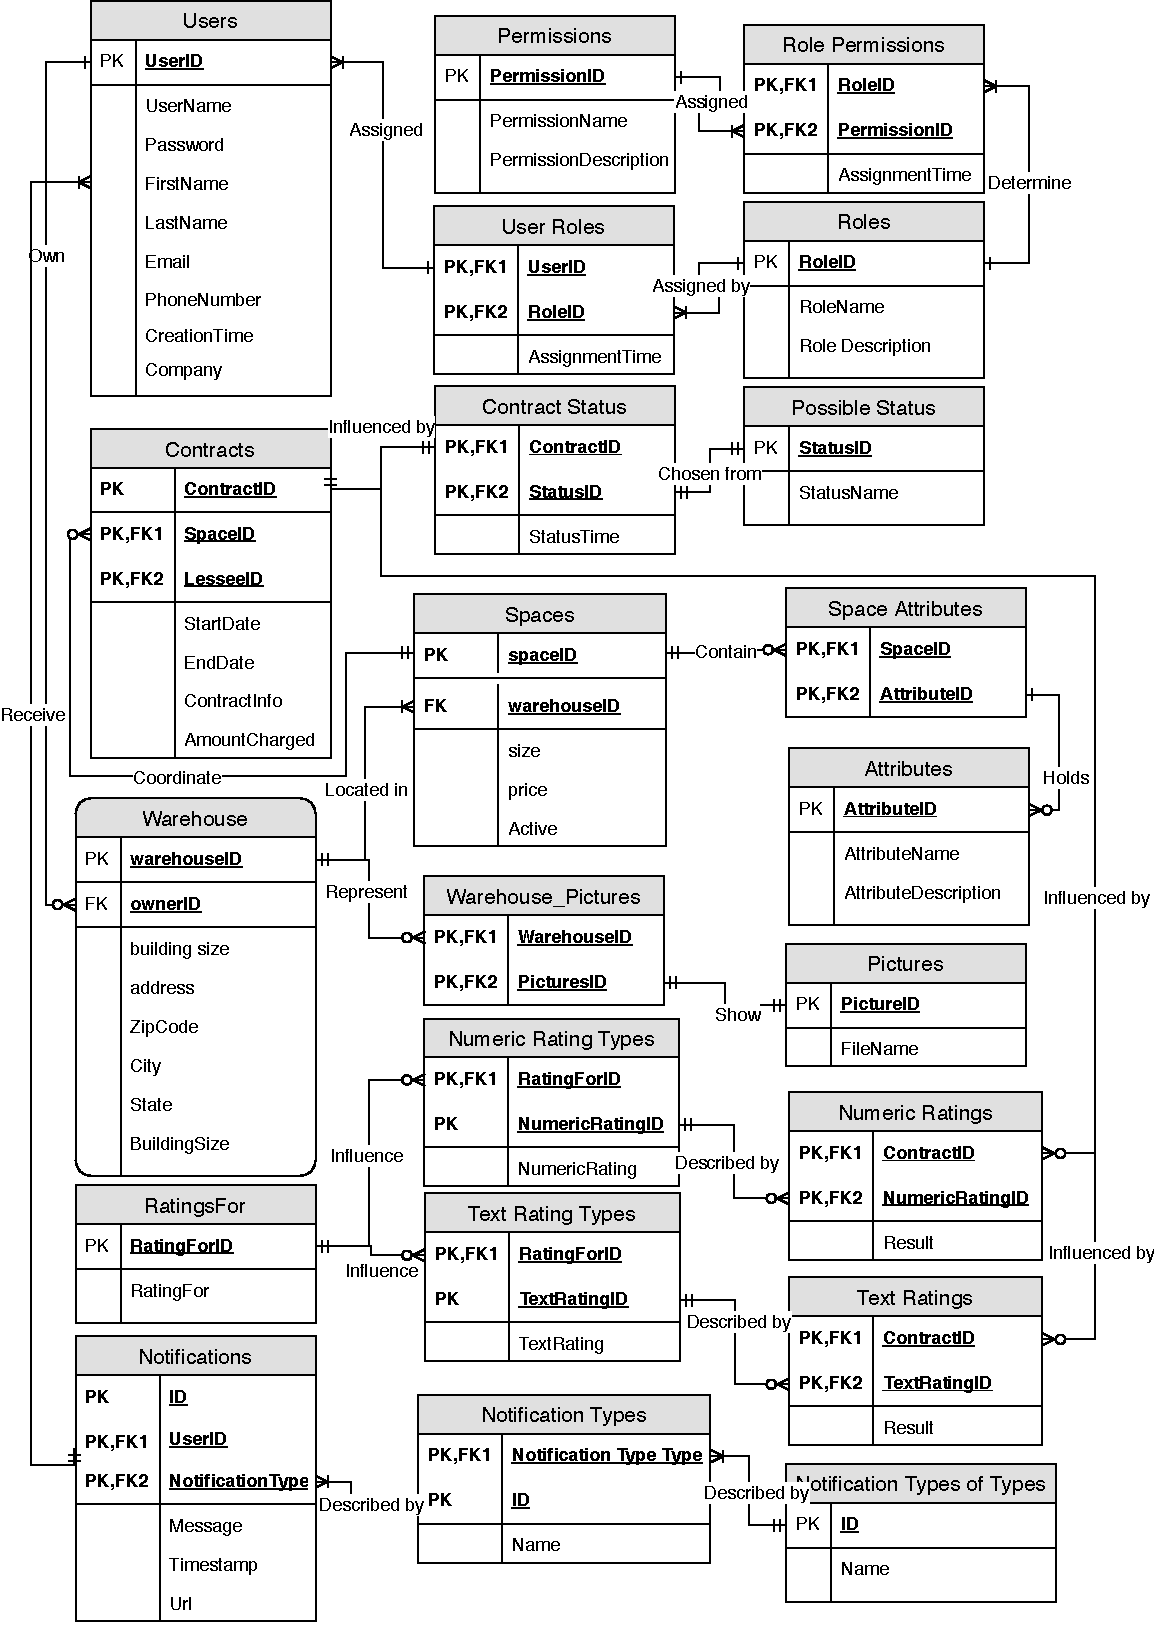
\includegraphics[page=1,width=.85\textwidth,height = .7\textheight]{Phase_3/ER_Diagram.pdf} 
\caption{Entity-Relationship Diagram}
\end{figure}

\pagebreak
\section{Ranking Algorithm}

\subsection{Utilization}
The ranking algorithm's dependency on utilization considers all the previous and future contracts for a designated space.  Utilization is divided into two parts, future utilization and past utilization.  The utilization equation is displayed in Equation~\ref{fig:utilization}.  This equation take the proportion between the time until or since the contract over the length of the contract.  This strategy promotes spaces that have not had a contract in a long time, and spaces that have shorter contracts.  Therefore the algorithim distributes contracts to a greater portion of the @Capacity community because this algorithm will distribute a higher score to less used space spaces.


\begin{figure}[h]
\[\text{Utilization} = \frac{\text{Time Until or Since the Contract}}{\text{Contract Length}}\]
\caption{Utilization for Contracts}
\label{fig:utilization}
\end{figure}


\subsection{Score}

The total score used by the ranking algorithm is a composite of 4 scores: distance, price, utilization and size.  Each one of these scores has an associated scale factor that can be changed based on the importance of each factor.  By default all the scores are scaled the same.  The total score is a simple weighted addition of each of the 3 factors as described below.



\subsubsection{Distance}

The distance score is calculated on line 287-297 in the "www/includes/rankingFunctions.php" file.  Distance\textunderscore away is a measure of how far away a given warehouse is from the clients given location.  Max\textunderscore distance\textunderscore wanted is maximum distance away a client wants their potential warehouse.  The equation below gives a linearly decreasing score to each warehouses based on its distance from the client defined location.  

\begin{figure}[h]
\[\mathrm{distance\_ score\ }=\mathrm{\ scale\ }\ast\ \left(1\ -\ \frac{(\mathrm{distance\_ away})}{(\mathrm{max\_ distance\_ wanted})}\right)\]
\caption{Distance ranking score}
\label{fig:dist}
\end{figure}

\subsubsection{Price}

The price score is calculated on line 322-326 in the "www/includes/rankingFunctions.php" file.  Space\textunderscore price is the cost of a given space.  Min\textunderscore price is the price of the cheapest space that fits the client's needs.  Max\textunderscore price is the price of the most expensive space that fits the client's needs.  The equation below gives the most expensive warehouse a score of 0, the least expensive a score of 1, and every warehouse in between a linear score between 0 and 1.

\begin{figure}[h]
\[\mathrm{price\_ score}\ =\mathrm{\ scale\ }\ast\left(1\ -\ \frac{\left(\mathrm{space\_ price\ }-\mathrm{\ min\_ price}\right)}{\left(\mathrm{max\_ price}\ -\ \mathrm{min\_ price}\right)}\right)\]
\caption{Price ranking score}
\label{fig:price}
\end{figure}

\subsubsection{Size}
The size score is calculated on line 299-320 in the "www/includes/rankingFunctions.php" file. Space\textunderscore score is the score given for each space in a warehouse. Max\textunderscore size represents the max size that each individual space has available for rent. Space\textunderscore size is user inputted value for their desired space size. This equation gives a linearly decreasing score to each warehouses based on its difference from the lessee defined size.  

\begin{figure}[h]

\[\mathrm{size\_ score}\ =\text{scale} * (1-\frac{\text{SpaceSize} - \text{SizeWanted}}{\text{MaxSpaceSize}})\]
\caption{Size ranking score}
\label{fig:size}
\end{figure}
\newpage
\section{Synthetic Data Generation}

\textbf{Contracts Pseudocode}
\\The code pertaining to the following pseudocode can be found on lines 302-362 on the file FINAL DATA GENERATION.R within the dataGeneration folder
\begin{enumerate}
\item Designate how many contracts are to be generated.
\item Generate a random number between 1 and 1400 (1400 being the number of spaces) to assign a space ID to each contract that is to be generated. 
\item Generate a random number between 350 and 1000 (this range being the range of lessee user IDs) to assign a lessee ID to each contract that is to be generated. The reason the random number is generated between 350 and 1000 is because 400-1000 are lessee user IDs, 1-350 are owner IDs, and 350-400 is a mixture of lessee and owner IDs.
\item Sort all space IDs in increasing order.
\item For each contract, if the current space ID is equal to the previous space ID, set the contract's start date equal to a random date that is greater than or equal to the previous contract's end date.
\item If the current space ID is different than the previous space ID, set the current contract's start date to a random date.
\item Set the end date for each contract to a date greater than the start date by a random number of days ranging from two weeks to two years.
\item Calculate the amount charge: for each contract, multiply the space's price/square foot/month by the length of the contract in months, the space's size, and the service fee.
\item Generate the contract information for each contract by pulling one string of random storage information from a list of storage items.
\item Compile the space ID, lessee ID, start date, end date, amount charged, and contract information into a data frame.
\item Write the contract data to a CSV file
\end{enumerate}
An important aspect to synthesizing random data that is also realistic is creating realistic contracts, as contracts are the entity that tie the space and lessee together. A realistic contract is a contract that is assigned to a particular space and lessee, does not overlap with another contract in the same space, lasts for a reasonable time, has a price calculated based on size and time, and contains information on what is being store. For this data, each contract is assigned to a space and lessee randomly using a simple "sample" function over the range of possible values for each attribute. The price is calculated using the space price and space size calculated during the space data generation. In this case, it was important to ensure that the price and size that were being used in each contract's price calculation corresponded to the space that the contract was being assigned to.\\
\\Another extremely important issue in creating realistic contracts was the scheduling aspect. As previously stated, realistic contract data contains start date and end dates that do not overlap for the same space. In order to prevent this from happening, the same logic that was used in the scheduling algorithm was applied to creating this data. This entails checking to see if a proposed contract's start date is before an existing contract's end date. In essence, this means contracts do not get assigned to spaces with outstanding contract requests. 




\end{document}